\documentclass[11pt,a4paper]{article}
\usepackage[english]{babel}
\usepackage[utf8]{inputenc}
\usepackage{verbatim}
\usepackage{amssymb}
\usepackage{graphicx}
\usepackage{wrapfig}
\usepackage{color}
\usepackage{a4wide}
\usepackage{subcaption}

\title{BW4T3 Instructions}
\date{\today}

\begin{document}

\begin{titlepage}
    \centering
    \vfill
    {\bfseries\Large
        BW4T3 Instructions\\
        \vskip2cm
        W. Pasman, M. B. van Riemsdijk, \\
    }    
    \vfill
    
\includegraphics[width=4cm]{TUD.png}
    \vfill
    \vfill
\end{titlepage}

\tableofcontents

\newpage

\section{Introduction}
Blocks World for Teams (BW4T) is a testbed for team coordination. BW4T allows for games with human-human, agent-agent and human-agent teams of variable sizes. The goal is to jointly deliver a sequence of colored blocks in a particular order as fast as possible. A complicating factor is that the players cannot see each other.

BW4T is a client-server system. The server is responsible for the administration, simulation and visualization of the virtual world: it keeps track of robots, rooms, blocks, connected GOAL agents, etc. The server uses Repast, software to simulate virtual environments, to do part of this administration. The client is GOAL, which runs a multi-agent system (MAS) and connects to the server. The agents in the GOAL client get percepts from the server, and send actions to the server. Client and server can run on a different computer. This document describes how to install the BW4T server, configure it, place the BW4T client in GOAL, configure the MAS file, and run the system.

This chapter descibes how users can install and use the Blocks World for Teams environment. For developer information please go to the project page on github  https://github.com/eishub/BW4T and click on the Link to Developer Details.

We use the following names to refer to directories of BW4T:
\begin{itemize}
\item $<$GOAL$>$ refers to the directory where you installed GOAL.
\item $<$SERVER$>$ refers to the directory where you have put the server.jar, documentation and utilities.
\item $<$CLIENT$>$ refers to the directory where you have put the client.jar.
\end{itemize}

\subsection{System requirements}
To use BW4T you need Java JDK 7 or higher. The BW4T3 environment has been tested on Windows 7, Windows 8 and OSX. Note that OSX may come with java 6 pre-installed. You need to install java 7. You can then keep java 6 installed as well, but ensure that java 7 is used as the default.

\subsection{Installation}
This document describes how to install Blocks World For Teams (BW4T) for use with GOAL. We briefly comment where necessary how it would work with a different agent system. You can also use BT4T stand-alone but this is not described in this document. 

You need to install a number of items to run BW4T from GOAL. 
\begin{enumerate}
 \item (if not yet done): Install Java 7 (download from http://www.java.com) and made it the default Java (such that double clicking on a jar makes it open with Java 7).
 \item You can download GOAL from $http://ii.tudelft.nl/trac/goal$. You can choose for the plugin for Eclipse or the stand-alone SimpleIDE.
 \item GOAL provides a sample Multi-agent-system 'BW4T3' that is demonstrating the Blocks World for Teams system. \footnote{If you run in a different agent system, you can download the client-side environment from $https://github.com/eishub/BW4T/releases$. Select $bw4t-client-X.Y.Z.jar$. This is the environment that should be attached to your agent system. You then will have to write your own agents that can run in the BW4T world.}
 \item You can download the BW4T server from $https://github.com/eishub/BW4T/releases$ and save it in $<$SERVER$>$. Select the latest $bw4t-server-X.Y.Z.jar$.
 \item You can optionally download the BW4T map editor from $https://github.com/eishub/BW4T/releases$ and save it in $<$SERVER$>$. Select the latest $bw4t-environment-store-X.Y.Z.jar$.
 \item You can optionally download the BW4T scenario editor from $https://github.com/eishub/BW4T/releases$ and save it in $<$SERVER$>$. Select the latest $bw4t-scenario-editor-X.Y.Z.jar$.
\end{enumerate}
  

\section{Running the server}
Run the server before running the client, as otherwise the client cannot connect to the server. Start the server by opening (typically: double clicking) the server.jar in $<$SERVER$>$. This should open the server window (Figure  \ref{fig:ServerWindow}). Note that during this opening, two other maps are created: 
\begin{itemize}
\item Maps: The folder in which all possible maps are put.
\item Log: The folder in which all log files will be placed.
\end{itemize}


\begin{figure}[!h]
\begin{center}
   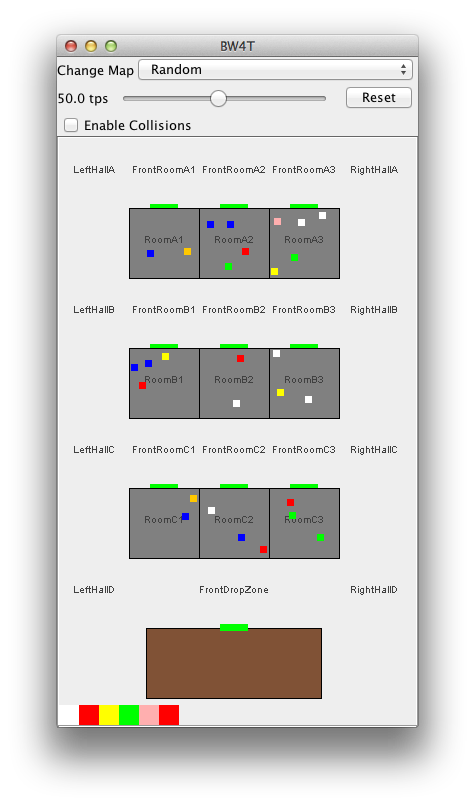
\includegraphics[height=10cm]{server.png}
   \caption{Server window}\label{fig:ServerWindow}
\end{center}
\end{figure}


\subsection{Advanced server settings}
The default settings for the server can be changed in the command line of your OS. 

For example, to change the server ip and/or server port  999 execute the following:

java -jar bw4t-server.jar -servip $<$server ip here$>$ (default: localhost) -serverport 999

The server will now start using the new values.

These are all the  options for the server:
\begin{itemize}
\item -scenario The path to the scenario folder required by repast. Default is BW4T.rs. We recommend to not change this.  
\item -map the name of the map file in the /maps/ folder (which is created at startup if it does not yet exist). Default is 'Random'. These are really xml files that you can create and edit with the map editor.
\item -serverip The ip to bind this server to. Default is 'localhost'. If you change the serverip and/or serverport, change the client settings correspondingly (see below). 
\item -serverport  The port to bind this server to. Default is 8000. You can change this if there already is another service on your machine using the default port. Make sure that you also set up the client accordingly if you change this.
\item -msg the message to be made available to the clients.
\item -gui true if GUI should be enabled, false if server should run without GUI. Defaults to true. Setting this to false  may be useful particularly for batch runs.
\item -key The key necessary to remotely kill the server
\item -collision whether the environment should check the collisions. Defaults to false. Note that collision checking still has some issues.
\item -paths True if draw paths is enabled. This allows you to see planned paths for entities.
\end{itemize}

\section{Running the client (Human Controlled Bot)}
Before running the client, make sure you have already started the server. Start (e.g., double click) the client.jar in $<$CLIENT$>$. Figure \ref{fig:Client} will show up and the bot is automatically added to the server. You can now control the bot by clicking (left or right) at different spots in the Client. Please refer to Section  \ref{ch:usingHI} for details on using the this client.

Notice: if you run both agents and human controlled bots, you should use the HUMANGUI option and launch the human GUIs in coordination with the agent platform. Please refer to the Advanced run settings below.

\begin{figure}[!h]
\begin{center}
  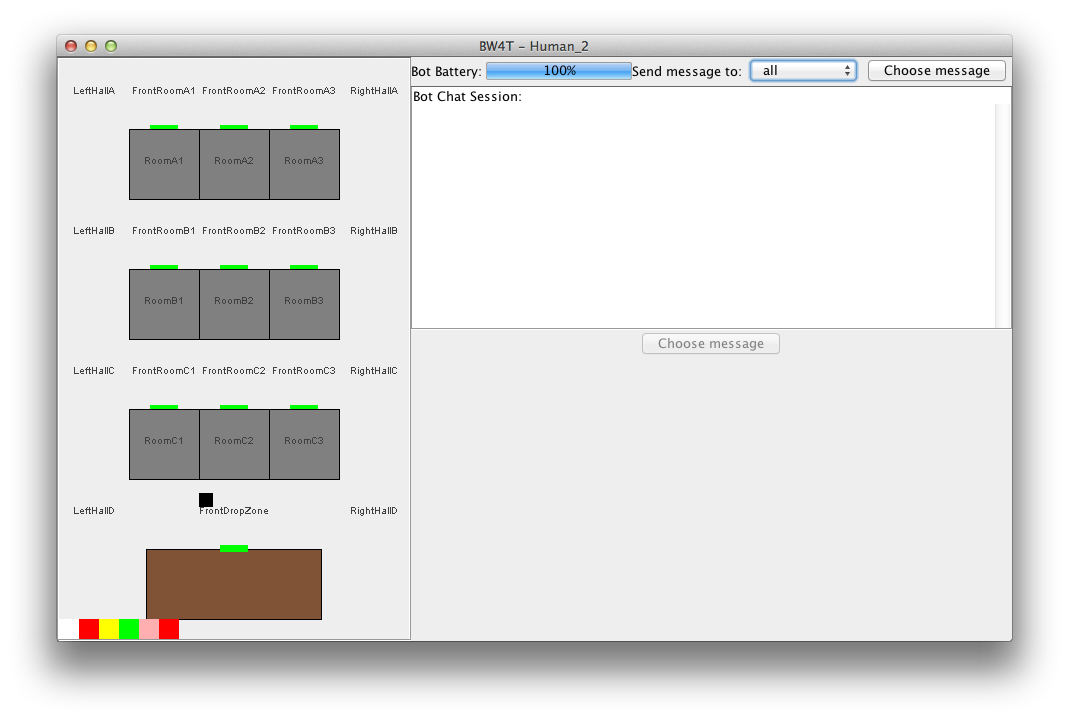
\includegraphics[width=0.5\textwidth]{HumanPlayerGUI/hpg.png}
  \caption{Client window}\label{fig:Client}
\end{center}
\end{figure}


\section{Running the client (Agent Controlled Bot)}
Before running the client, make sure you have already started the server. Start your favourite Agent platform and load run the MAS. If you use GOAL, this means open the .mas2g file and press the run button. This time, no new windows will appear. The agent will control your bot,  and agent behaviours can be seen only by introspecting the agents with your agent platform tools. In the server window you will see your bot(s) move according to the rules applied in the .goal file(s).

\subsection{Advanced run settings}
\label{sec:clientadvancedrunsettings}
The following MAS init parameters are available (the default values are shown inside the brackets). These init parameters should be placed inside the config.xml file. 

The HUMANGUI option is needed if you have a human GUI connected with an agent (and the agent should receive percepts as well).

In GOAL these settings can be changed also from the mas2g file. The CONFIGFILE option is the only needed option in the MAS file, if you use a config file.  

\begin{itemize}
\item

    CLIENTIP("localhost"):    client's own IP. Passed to server so server is able to find us with this IP. 

\item
    CLIENTPORT("2000"):   The port that the client listens to. 


\item
    SERVERIP("localhost"):
 The IP address of the server. 
  
\item
    SERVERPORT("8000"):
   The Port that the server listens on. 

\item
    AGENTCOUNT("0"):
 the amount of agents (also specified in the launchpolicy section, see below), that the client should load. If the agentcount is higher than the amount of entities in the map then they won't be loaded. (default: 0).. 
    
\item
    LAUNCHGUI("true"):
    whether to launch a separate GUI for each bot (controlled by an agent or human) can be set to true or false. This GUI shows the environment from the perspective of the bot. (default:false).When this option is used, the human GUI is connected with the agent platform. A special agent in the agent platform can then communicate with the HumanGUI using entity actions that are available specifically for this purpose. This way, a human player can be a fully qualified player in the agent platform (e.g., use the native communication mechanisms in the agent platform).


\item
    HUMANCOUNT("1"):
    the amount of human players that should be loaded. If the humancount is higher than the amount of entities in the map then they won't be loaded. 

\item
    AGENTCLASS("nl.tudelft.bw4t.client.agent.BW4TAgent"):
    The java agent class to load when new entities appear.
   

\item
    GOAL("true"):
    are we connected with GOAL? This param should be auto detected, it will be set to false if the program is started from commandline.

\item
    KILL(""):
  The key we should try to use to kill the remote server.
 
\item
    CONFIGFILE(""):
    The file from which the client reads the configuration. This is an xml file that can be generated with the scenario editor. The file is read relative to the directory containing the client environment jar file, unless you use an absolute path. It is recommended to place the xml relative to the client environment location, and not use an absolute path. WARNING: currently the scenario editor exports MAS files with absolute paths. You need to fix this manually.
 
\item
    GOALHUMAN("false"):
    Forces the use of the human GUI with an GOAL agent to translate the commands. You should turn on this option if you have a human GUI but still want the agent to receive the percepts.

\item
    MAP(""):
    The map name to be loaded. If you specify a map, the server will reset to load the new map, which disconnects all entities.
     
\item    
    SPEED(""):
    The speed (fps) at which the simulation runs on the server. Must be between 5 and 100. If left empty, the server will keep its current setting.

\item    
    LOG("ERROR"):
    The log4j log level to be used. Available values: OFF, FATAL, ERROR, WARN, INFODEBUG and ALL.

\end{itemize}


\section{Using the Server Interface}
The server interface (Figure \ref{fig:ServerWindow}) offers very limited controls, as the main control is running through software (the agents, management system, buttons and settings in the agent platform). There are only 3 controls available:
\begin{itemize}
\item{Reset}: By pressing this button, the environment is completely killed and restarted, all entities are killed (which kicks out all agents), the map is reloaded from scratch. We recommend killing from your agent platform as that offers the agent platform the opportunity to handle this take-down in a nice way.
\item{Enable Collisions}: When enabled, bots can collide with each other. When disabled, they can run over each other without any interference. We recommend to keep this \emph{disabled} as this option is not yet fully supported (you may have problems with path planning).
\item{Change Map}: By selecting a map, you effectively \emph{Reset} the system, to restart it with a different map.
\end{itemize}





\section{Using the Human Player GUI}\label{ch:usingHI} 

When the GUI is open (Figure \ref{fig:humanPlayerGUI}), two main parts can be seen:
\begin{enumerate}
\item left: the map area, where the map and the block sequence are being displayed.
\item right: the message area, where messages between bots and e-partner are being displayed.
\end{enumerate}

The name of the bot that is controlled is shown in the title bar of the GUI.

\begin{figure}[h]
\begin{center}
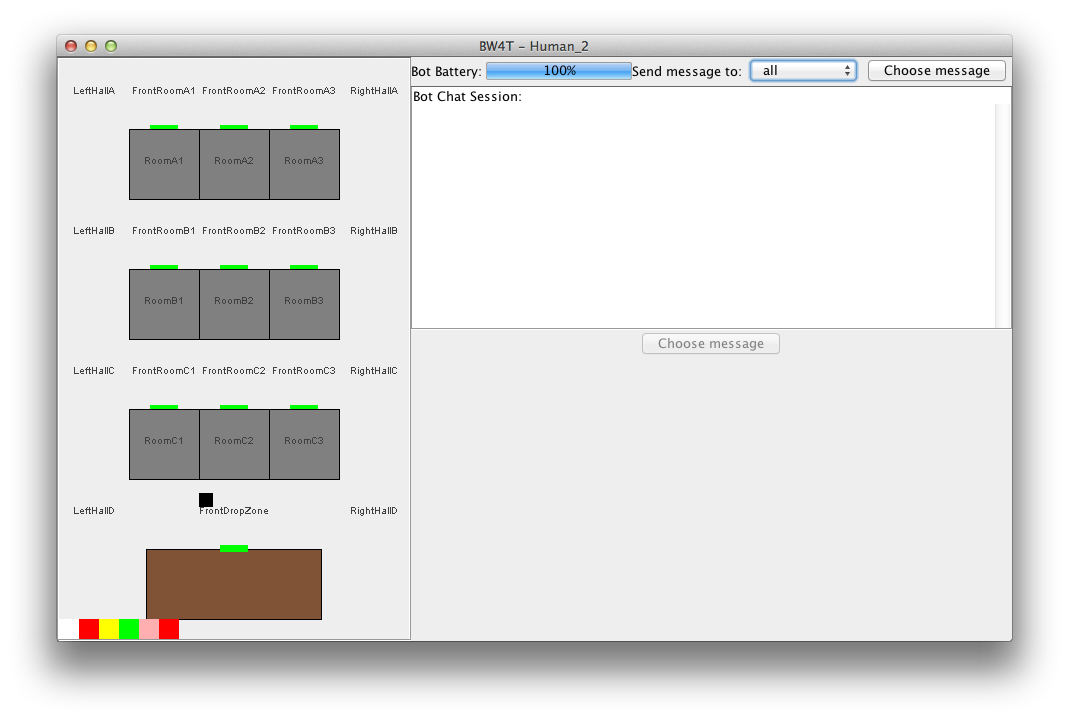
\includegraphics[width = 0.8\textwidth]{HumanPlayerGUI/hpg.png}
\caption{Human Player GUI with map panel (left) and message panel (right).}
\label{fig:humanPlayerGUI}
\end{center}
\end{figure}

\subsection{General use}
To use the human player interface, the user clicks with the left (occasionally the right) mouse button in the GUI. Depending on where the user clicks, different menus appear. The user then picks the appropriate action from the menu to execute that action. In the following sections the possibilities are explained.

In the map area, the bot can be directed by clicking on the map. Different pop-up menus will appear upon clicking on different entities on the map.

In the message area, the remaining battery charge of the bot  is shown in the top left. The combo box in the top center allows the user to select other bots, to which which messages can be sent. The top right 'Choose message' button allows the user to select a message to send.

The text area in the center shows the previous messages that were communicated.

The map panel shares the message target with the message panel. So all messages that are sent from the map panel are sent using the actual message target setting in the message panel. A message will be send to all bots by default. Please refer to the Message Panel section below to adjust the receiver(s) of messages.

\subsection{Map Panel}
A picture of the Map Panel is shown in Figure \ref{fig:mapPanel}.

\begin{figure}[h]
\begin{center}
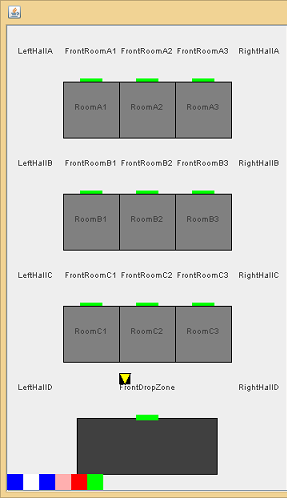
\includegraphics[width= 0.3\textwidth]{HumanPlayerGUI/hpg-left.png}
\end{center}
\caption{Map Panel}
\label{fig:mapPanel}
\end{figure}

Here the following actions can be done:

\begin{itemize}

\item \textbf{Go to: $"place"$}:
To command the bot to go to a room or a certain place in the corridors, click on the room or place where the bot needs to go to. The corridor menu (figure ~\ref{fig:corridorMenu}) will appear next to your mouse pointer with the option $go$ $to$ $here$ or $Go$ $to$ $"room"$.\\

\begin{figure}[h]
\centering
\begin{minipage}{0.48\textwidth}
	\centering
	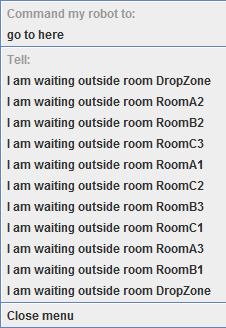
\includegraphics[width=0.5\textwidth]{HumanPlayerGUI/hpg-corridor-menu.png}
	\caption{Corridor menu}
	\label{fig:corridorMenu}
\end{minipage}\hfill
\begin{minipage}{0.48\textwidth}
	\centering
	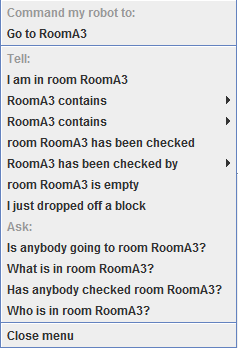
\includegraphics[width=0.5\textwidth]{HumanPlayerGUI/hpg-room-menu.png}
	\caption{Room menu}
	\label{fig:roomMenu}
\end{minipage}
\end{figure}


\item \textbf{Send message: I am waiting outside $"room"$}:
To send a message to a bot or to all bots, click in the corridor. The corridor menu (figure ~\ref{fig:corridorMenu}) will appear next to your mouse pointer with the options $I$ $am$ $waiting$ $outside$ $"room"$. 

\item \textbf{Send message: I am in $"room"$}:
To send a message to a bot or to all bots, click in the room. The room menu (figure \ref{fig:roomMenu}) will appear next to your mouse pointer with the option: I am in $"room"$. 

\item \textbf{Send message: tell other bot(s) $"information"$}:
To send a message to a bot or to all bots with certain information about a certain room, click on the room. The room menu (Figure \ref{fig:roomMenu}) will appear next to your mouse pointer with the messages you can send.

\item \textbf{Send message: tell other bot(s) about blocks}:
By clicking on a block (particularly, those below the drop zone), the user can tell a bot or all bots something about that block, or ask others for information about that block.

\item \textbf{Send message: ask other bot(s) $"question"$ about certain room}:
To ask a bot or all bots a question about a certain room, click on the room. The room menu (Figure \ref{fig:roomMenu}) will appear next to your mouse pointer with the possible questions that can we asked.

\item \textbf{Pick up block}:
To pick up a $"block"$, click on the block that needs to be picked up. The block menu (Figure \ref{fig:blockMenu}) will appear next to your mouse pointer. Click on $Go$ $to$ $"color"$ $block$. When the controlled bot is standing on the block, click on the bot. The block menu when standing on block (Figure \ref{fig:blockMenu2}) will appear. Click on $Pick$ $up$ $"color"$ $block$.

\begin{figure}[h]
\centering
\begin{minipage}{0.5\textwidth}
\centering
  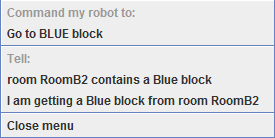
\includegraphics[width=.8\linewidth]{HumanPlayerGUI/hpg-block-menu1.png}  
  \caption{Block menu} \label{fig:blockMenu}
\end{minipage}\hfill
\begin{minipage}{0.5\textwidth}
  \centering
  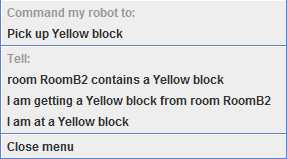
\includegraphics[width=.8\linewidth]{HumanPlayerGUI/hpg-block-menu2.png}
  \caption{Block menu when standing on block} \label{fig:blockMenu2}
\end{minipage}
\end{figure}

\item \textbf{Drop block}:
To drop the block that is currently being held, click on the room in which it needs to be dropped. The room menu when holding block will appear next to your mouse pointer. This menu is almost identical to (Figure \ref{fig:roomMenu} but it has an extra item 'Put down block'). Click on $Put$ $down$ $block$. Do note that the controlled bot should be in the same room as where you want to drop the block.


\item \textbf{Pick up e-partner}:
To pick up an e-partner, click on the e-partner that needs to be picked up. The e-partner menu (Figure \ref{fig:epartnerMenu}) will appear next to your mouse pointer. Click on $Go$ $to$ $e-partner$. When the controlled bot is standing on the e-partner, click on the e-partner again. The e-partner menu when standing on e-partner (Figure \ref{fig:epartnerMenu2}) will appear. Click on $Pick$ $up$ $e-partner$.

\begin{figure}[h]
\begin{minipage}{0.48\textwidth}
  \centering
  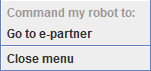
\includegraphics[width=.5\linewidth]{HumanPlayerGUI/hpg-epartner-menu1.png}
  \caption{The e-partner menu}
  \label{fig:epartnerMenu}
\end{minipage}\hfill
\begin{minipage}{0.48\textwidth}
  \centering
  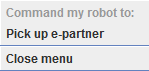
\includegraphics[width=.5\linewidth]{HumanPlayerGUI/hpg-epartner-menu2.png}
  \caption{E-partner menu when standing on e-partner}
  \label{fig:epartnerMenu2}
\end{minipage}
\end{figure}

\item \textbf{Send message to e-partner}:
To send a message to the e-partner that is currently being held, click on the e-partner. The e-partner menu when holding e-partner (Figure  \ref{fig:epartnerMenu3}) will appear next to your mouse pointer. Click on $I$ $am$ $going$ $to$ $"room"$. This option will only appear if the e-partner has GPS enabled.

\begin{figure}
\begin{center}
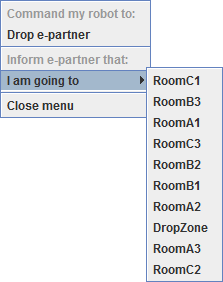
\includegraphics{HumanPlayerGUI/hpg-epartner-menu3.png}
\end{center}
\caption{E-partner menu when holding e-partner}
\label{fig:epartnerMenu3}
\end{figure}

\item \textbf{Drop e-partner}:
To drop the e-partner which is currently being held, click on the e-partner. The e-partner menu when holding e-partner (figure  \ref{fig:epartnerMenu3}) will appear next to your mouse pointer. Click on $Put$ $down$ $e-partner$.

\end{itemize}


\subsection{Message panel}
Figure \ref{fig:humanPlayerGUI} (right half) and \ref{fig:mp2} show the Message Panel. The second choose message button will only be enabled when the bot is holding an e-partner. Below this button, the e-partner chat session will appear when the bot holds an e-partner for the first time. Figure \ref{fig:mp2} shows the Message Panel when the e-partner has been held and dropped.

\begin{figure}[h]
\begin{center}
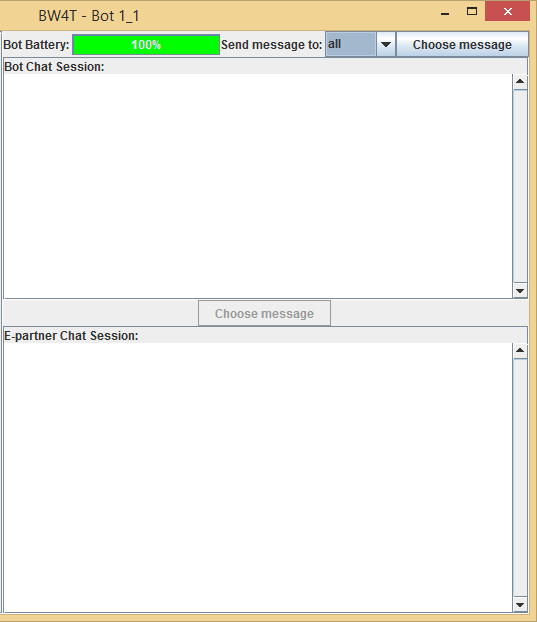
\includegraphics[width=0.5\textwidth]{HumanPlayerGUI/hpg-right-epartner.png}
\end{center}
\caption{Message Panel with e-partner section. Refer to Figure \ref{fig:humanPlayerGUI} for the panel without e-partner section. }
\label{fig:mp2}
\end{figure}

\begin{itemize}

\item \textbf{Select message receiver}
To select who a message needs to be sent to, click on the dropdown box (Figure \ref{fig:receiverDropDown}) at $Send$ $message$ $to:$. The receiver is by default $all$.
When set to $all$, all other bots receive the message. When set to a specific bot, only that bot receives the message.

\item \textbf{Send message to bot(s)}
To send a message, click on the $Choose$ $message$ button. A menu (Figure \ref{fig:messageBot}) will appear next to your mouse pointer with the possible messages to be sent.

\begin{figure}[h]
\begin{minipage}{0.48\textwidth}
  \centering
  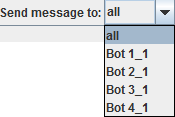
\includegraphics[width=0.6\textwidth]{HumanPlayerGUI/hpg-bot-receiver.png}
  \caption{Select receiver dropdown}
  \label{fig:receiverDropDown}
\end{minipage}\hfill
\begin{minipage}{0.48\textwidth}
  \centering
  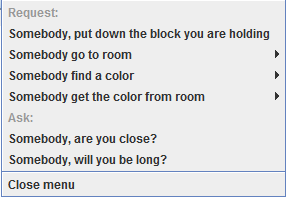
\includegraphics[width=0.6\textwidth]{HumanPlayerGUI/hpg-bot-message.png}
  \caption{Choose message button menu}
  \label{fig:messageBot}
\end{minipage}
\end{figure}


\item \textbf{Answer a question}
To answer questions asked by other bots, click in the bot chat session box. A menu (figure ~\ref{fig:answerBot}) will appear next to your mouse pointer with the possible answers to be sent.

\begin{figure}[h]
\begin{center}
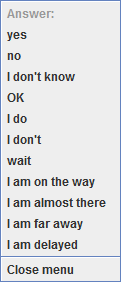
\includegraphics[width=0.14\textwidth]{HumanPlayerGUI/hpg-bot-chat.png}
\end{center}
\caption{Bot answer menu}
\label{fig:answerBot}
\end{figure}

\item \textbf{Send message to e-partner}
To send a message to the e-partner that is currently being held, click on the choose message button. A menu (Figure  \ref{fig:epartnerMenu3}) will appear next to your mouse pointer. Click on $I$ $am$ $going$ $to$ $"room"$. This option will only appear if the e-partner has GPS enabled.

\item \textbf{Drop e-partner}
To drop the e-partner that is currently being held, click on the choose message button. A menu (figure  ~\ref{fig:epartnerMenu3}) will appear next to your mouse pointer. Click on $Drop$ $e-partner$. The choose message button will be disabled after dropping the e-partner.

\end{itemize}



\section{Hints for GOAL users}
In this section we give some hints that are specific for using BW4T from the GOAL agent system.

\subsection{mas2g file}
The number of agents is specified at two places in the mas2g file. First, the agentcount and humancount specify the number of entities of the corresponding type that should be created in the environment. Second, the launchpolicy specifies which and how many agents should be connected to these entities. Make sure that the agentcount and humancount in the initialization parameters are in line with the launch policy section in the mas2g file. 
If you use BW4T from a batch runner, you may want to reset the server after each run. This is done by specifying a map in the mas file init parameters. See also Section \ref{sec:clientadvancedrunsettings}.

\subsection{Restarting, pausing and resuming the system}
If you are running from SimpleIDE, you can pause and resume the system at any time by clicking the pause or step buttons. 

When running from Eclipse, to be able to pause the system, don't run the mas2g file as described above. This time, open the mas2g file and click on the debug button (the small bug icon).

\begin{wrapfigure}{r}{0.5\textwidth}
  \begin{center}
    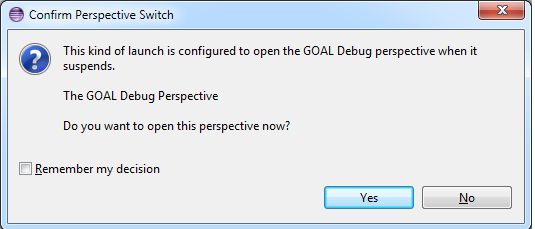
\includegraphics[width=0.5\textwidth]{debug.png}
  \end{center}
  \caption{Choose yes}\label{fig:EclipseDebug}
\end{wrapfigure}
Eclipse will ask you whether you would like to go to the debug screen (see Figure \ref{fig:EclipseDebug}), click yes and watch your screen adjust.
Now you can see the running bots listed at the left side, and the current goals, beliefs and knowledge of the selected bot on the right side. Beneath the list the goal file belonging to the bot is shown and at the bottom of the screen, all debug actions are being run (Figure \ref{fig:Eclipse}).
To pause the system, select the bot to be paused and click on the pause button. To resume, select the bot and click resume.
To restart the system, do the following
\begin{enumerate}
\item In eclipse, kill the MAS by clicking the red box (stop button) at the right of the console window.
\item In the server window, press Reset, or choose a new map from the Change Map menu.
\item Run the MAS in Eclipse as described above.
\end{enumerate}

\begin{figure}
  \begin{center}
    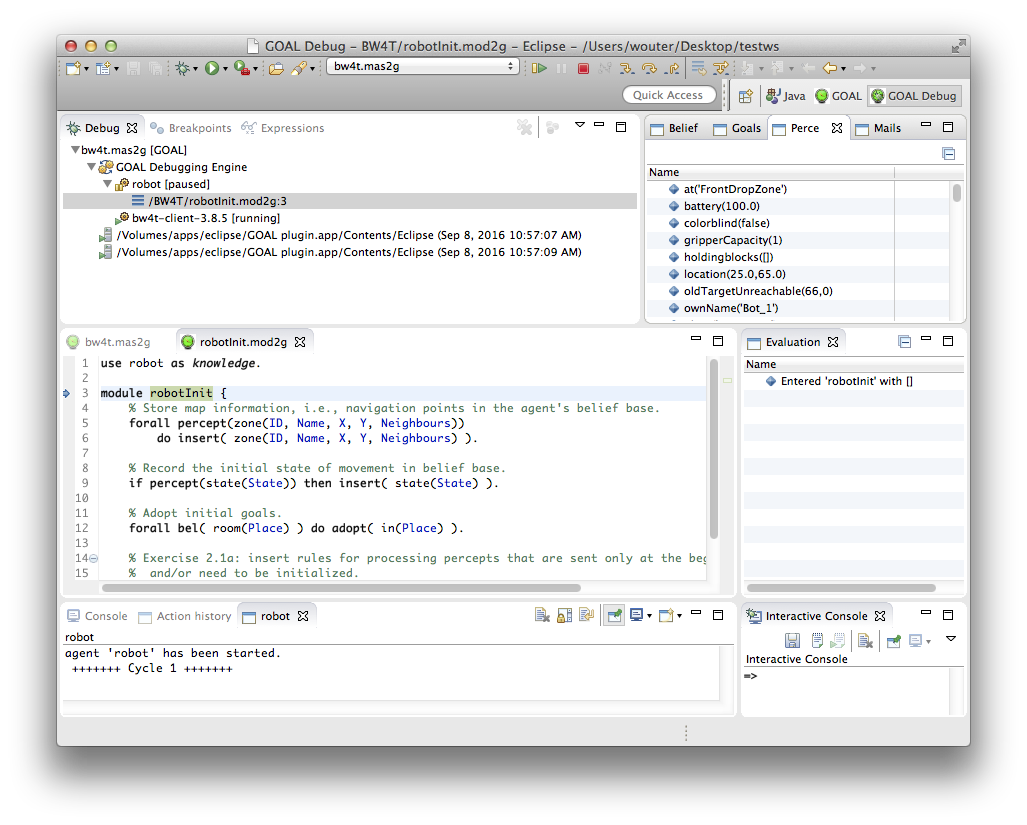
\includegraphics[width=0.8\textwidth]{debugmode.png}
    \caption{Debug mode}\label{fig:Eclipse}
  \end{center}
\end{figure}



\subsection{Running on multiple computers}
BW4T server can handle multiple clients out of the box. However, if you run multiple agent systems separately, agents in these separate platforms will not see each others' agents. 

To make a real distributed agent system where all agents can see each other, the agent system itself has to be run distributed. 

For GOAL, this is done as follows. You should designate one of these computer as the server. On this computer you can start the server as described in the first section of this guide. You must use RMI messaging (check the GOAL Run menu) to allow other GOAL runtimes to connect with the main GOAL instance that runs on the server.
You need to check a few things in the MAS that you use here:
\begin{itemize}
\item specify a map such that the environment resets when you start up the MAS
\item make sure that the map that is used has enough entities to accommodate all agents in all computers that want to connect
\item make sure that the entities get the proper type, by specifying the proper agentcount and humancount.
\end{itemize}
The other computers will then function as client. Create a MAS file for each of these, and configure this MAS as follows (see also bw4thuman.mas2g in the GOALagents directory of GOAL):
\begin{itemize}
\item set the serverip and serverport initialization parameters to the ones that the server is listening on (default for the server is localhost and port 8000).
\item Set the humancount and agentcount parameter on each client to reflect how many human or agent players that client should load.
\item Use humanbot.goal for human agents
\item use env = $<$CLIENT$>/$client.jar". in the environment section. Do not connect to an already running environment in another MAS. This is because BW4TClient creates GUIs for humanbots, on the machine where it is running.
\item Check that the launchpolicy picks up the proper entity type, so use 'human' if you want to attach to human entities etc.
\end{itemize} 

\subsection{Distributed Human GUIs}
This section describes how to run a set of distributed human GUIs such that they all communicate through GOAL. Before running a set of distributed Human GUIs with Eclipse, make sure that the server is installed on one machine. Furthermore, make sure that the server map can contain a sufficient number of entities.
To run a set of distributed Human GUIs with GOAL, do the following:
\begin{itemize}
\item Start the server
\item For each machine where you want to have a human GUI:
    \begin{enumerate}
    \item Start your agent platform (SimpleIDE or  Eclipse IDE)
    \item Open the MAS file of the bw4thuman.mas2g
    \item adjust the serverip to correctly point to the machine ip number where the server runs
    \item Start the MAS
    \end{enumerate}
\end{itemize}

\subsection{Programming a BW4T Agent}
To program your own BW4T agent, use the same actions as specified in the demorobot. You can  choose to change the pre- and post conditions of each action.

Percepts are retrieved automatically by GOAL, see the percept specifications for what percepts you can expect.

In order for messages received by other GOAL agents to appear on the GUI of your agent, you should add the following lines to your GOAL agent’s code:
\begin{enumerate}
\item Add the following line to your knowledge base:\\
\#import "messageTranslation".
\item Add the following line at the end of your goal file. \\
\#import "message.mod2g".
\item Add the following line to the start of your event module: \\
if bel(true) then message. \\
This will make sure that the message module that was just imported will be run first when entering the event module.
\item Your own message handling code should be performed after this line and should delete any messages after handling them. Otherwise they will be continuously posted to the GUI as they are not deleted by the message module. If you don’t do any message handling yet you can add the following line below the one provided in step 3 to delete all received messages: \\
forall bel(received(Agt,Msg)) do delete(received(Agt,Msg)).
\end{enumerate}

\subsection{Testing your agent}
In order to test your agent you should edit the bw4t.mas2g file as follows.
\begin{itemize}
\item Add your agent to the agentfiles list.
\item Add a line to the launchpolicy (copy the line of the demorobot and replace 'demorobot' with the name of your agent).
\end{itemize}
Make sure that you set GOAL to launch the desired number of your agent. Also make sure that the initialization parameter of agentcount is not set to 0 as then only humanbots will be loaded.

Note that besides in the bw4t.mas2g file, the number of agents is also specified in the map that you use. This number determines the maximum amount of bots that can appear on the map. If the maximum number of agents to be launched as specified in the bw4t.mas2g file is bigger than the number of agents specified in the map, some of the agents will not appear on the map and not be part of the team. 


\section{Log file}
Repast logs the following for each run into a file. The filename is “BW4TXXXX.log” where XXX is the date and time to make the filename unique. The file is saved in the $<$SERVER$>/$log directory. It contains:
\begin{enumerate}
\item sequence: goal sequence (which block colors are to be dropped)
\item room: initial blocks per room
\item action: log of each action of a bot, with timestamp 
\item total time: total time to complete task. Begin time is determined by first incoming action. End time is determined by the last block of the sequence dropped.
\item agentsummary: for each agent:
    \begin{itemize}
    \item the bot type containing its handicaps
    \item \# correct drops in dropzone
    \item \# incorrect drops in dropzone
    \item total time of standing still
    \item \# messages to other agents
    \item \# rooms entered
    \end{itemize}
\end{enumerate}
Logs are written to the file as soon as possible, so that information won't get lost when the system is being killed before the end of the sequence is reached.

\newpage

\section{Loading and creating new maps}
This section describes how you can edit existing maps or create new maps from scratch. This can be done with a editing tool, or by directly editing the map files manually.




\subsection{Using the Environment Store}
The Map Editor is a tool for editing maps for the BW4T server. Double click the jar file environment-store.jar  in the $<$SERVER$>$ directory to start the  editor.

\begin{wrapfigure}{r}{0.4\textwidth}
  \begin{center}
    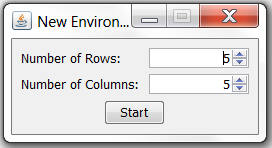
\includegraphics[width=0.4\textwidth]{EnvironmentStore/SizeDialog.png}
  \end{center}
  \caption{Choose the amount of columns and rows}\label{fig:MapSize}
\end{wrapfigure}


After starting up, the map size dialog (Figure \ref{fig:MapSize}) appears, which can be used as follows.
Here you can choose the amount of rows and columns you want the environment to consist of. Each cell in the "table" can be used to fulfill one piece of the map. This could either be a room, a corridor, a dropzone, a charging zone, start zone or a blockade. By pressing the colours at the bottom you can generate the sequence to be completed. This can also be done by pressing the according numbers on the keyboard. 

% we put the figure even ahead of the map editor section, to allow tex to be more flexible with
% the placement. Unfortunately tex keeps delaying the placement and we end up with a mess of pictures
% on one page with very little text remaining between the figures....
\begin{figure}
	\center
	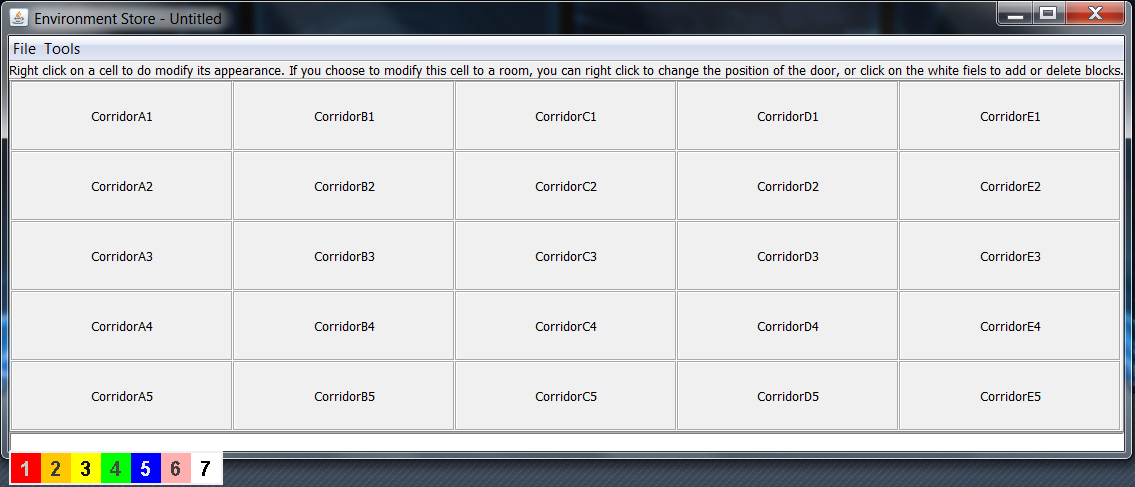
\includegraphics[scale=0.55]{EnvironmentStore/MapEditor.png}
	\caption{the map editor with a 5x5 freshly created map}\label{fig:MapEditor}
\end{figure}

At the moment, for an existing map to be loaded in the map editor, the correct sizes of the map have to be entered before the map can be loaded.

In the Map editor GUI above you can add blocks to rooms. To add blocks to rooms, right click in the cell, adjust the type of the zone to Room. Now you can add blocks the way you did with the sequence. Right clicking the cell again lets you choose at which side of the room you want the door. When you're done, press save. 
By pressing Tools in the menu bar, you are able to randomize zones, blocks and sequences. WARNING: Randomizing these will not always guarantee that the sequence can be completed.
By pressing File in the menu bar, you are able to watch a preview of your map, and you are able to save the map. Save the map in the $<$SERVER$>/$maps folder \footnote[1]{This map directory appears after the first run of the server.}.  


\begin{wrapfigure}{r}{0.3\textwidth}
  \begin{center}
	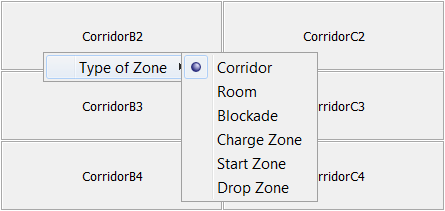
\includegraphics[width=0.3\textwidth]{EnvironmentStore/DropDownMenuRoom.png}
  \end{center}
  \caption{the drop down menu generated when a zone is right clicked}\label{fig:DropDownMenuRoom}
\end{wrapfigure}

\subsection{Map editor}
After specifying the amount of rows and columns the map should have, and clicking on the Start button, 
the map editor is launched. Figure \ref{fig:MapEditor} shows the environment store after launch, with a 5x5 map.

The map editor has many functionalities. The functionalities are detailed bit by bit in this documentation.


\subsection{Editing a room}

Right click on any corridor (or any zone of the matrix for that matter), and the drop down menu is shown (Figure \ref{fig:DropDownMenuRoom}).

This allows a zone to be converted to any one of a corridor, a room, a blockade, a charge zone, a start zone, and a drop zone. The following figure shows the different appearances of the zones in the map editor (Figure \ref{fig:DifferentRooms}).

As can be seen, The room and drop zone contain a green border. This is to indicate which way the door to enter the room is faced. This is also editable. When right clicking on a certain room, a drop down menu pops up (Figure \ref{DropDownMenuRoom2}).



 \begin{figure}
        \centering
        \begin{subfigure}[b]{0.5\textwidth}
		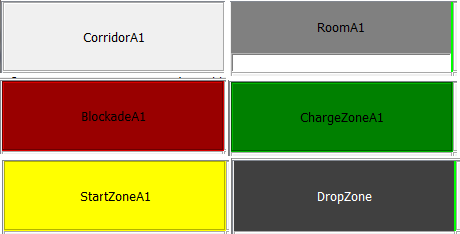
\includegraphics[width=0.9\textwidth]{EnvironmentStore/DifferentRooms.png}
		\caption{the color palette at the bottom of the map editor}\label{fig:DifferentRooms}
        \end{subfigure}%
        \begin{subfigure}[b]{0.5\textwidth}
	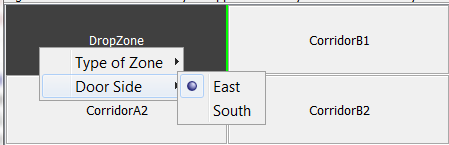
\includegraphics[width=0.9\textwidth]{EnvironmentStore/DropDownMenuRoom2.png}
	\caption{the drop down menu generated when a room is right clicked}\label{DropDownMenuRoom2}
        \end{subfigure}
        \caption{Drop Down menus}\label{fig:animals}
\end{figure}




This drop down menu lists the directions the door can face while still being accessible. In this case, as it is the top left zone, only doors facing east or south are possible.
\subsection{Editing a sequence}
Under the zones of the map editor is a white rectangle that contains the sequence for that map. This same rectangle is also present in the rooms that aren't drop zones. The rectangles are given here:
\begin{center}
	\centering
	
\includegraphics[scale=0.5]{EnvironmentStore/SequenceEditor.png}\\
	Figure 6: The rectangle at the bottom of both the map editor and the rooms.
\end{center}
The rectangle in the rooms can be used to enter colors, which are then used in the blocks that are placed in that room. The rectangle under the zones can be used to enter the colors that make up the sequence that has to be completed for that map. To add colors, the color palette is useful.
\subsection{Color palette}
At the bottom of the map editor is the color palette. A larger picture is given in figure 7:
\begin{center}
	\centering
	
\includegraphics{EnvironmentStore/ColorPalette.png}\\
	Figure 7: the color palette at the bottom of the map editor
\end{center}
The color palette is used for adding blocks to rooms and the sequence to be completed in the map. When clicking on the box containing either the sequence of the map or the blocks in the room, the color palette is shown. It allows for the adding of colors by clicking on the respective colors on the palette, but colors can also be added by entering the respective numbers in the colors (pressing 1 adds a red block to the room or sequence, for example) and also by entering the first letter of the color (so pressing R adds a red block).
\subsection{File menu}
The file menu contains not only the standard operations for exporting a created map to a file, so that it can be used later, but also a few other options. The drop down menu is as follows:
\begin{center}
	\centering
	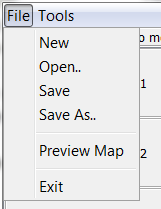
\includegraphics{EnvironmentStore/DropDownFile.png}\\
	Figure 8: the drop down menu created when the 'File' menu item is clicked
\end{center}
The New-, Open...-, Save- and Save as...-options are the standard file operations and need no further explanation. However, as added functionality to the options, it is impossible to save a map not containing either a start- or drop zone, as well as a map not containing a block in its sequence, and saving an unsolvable map will give a warning describing what's wrong. The Exit-option also needs no further explanation. The Preview-option gives a preview of the created map, as how it would be rendered when used as an actual map for bots. For a non-edited 5x5 map, the preview looks as follows:
\begin{center}
	\centering
	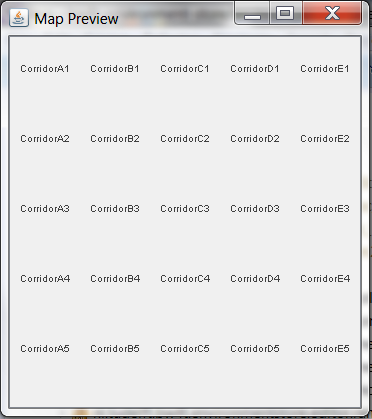
\includegraphics{EnvironmentStore/Preview.png}\\
	Figure 9: The preview of a 5x5 non-edited map, with no blocks in the sequence
\end{center}
\subsection{Tools menu}
The other drop down menu at the top of the map editor is the tools menu. This menu contains options to use several tools. The drop down menu is given here:
\begin{center}
	\centering
	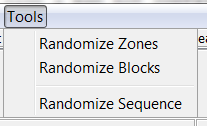
\includegraphics{EnvironmentStore/DropDownTools.png}\\
	Figure 10: The drop down menu created when the 'Tools' menu item is clicked.
\end{center}
Clicking on the 'Randomize Zones' option creates a random map, based off a vanilla map with reclassification of rooms to blockades, charge zones or corridors, and with reclassifications of existing corridors to charge zones. The map is always solvable, given that all the blocks in the sequence are present in the map and no further changes are made to the map. The 'Randomize Blocks' option randomizes the blocks contained in every room according to parameters that the user has to specify. The interface for specifying the parameters is given here:
\begin{center}
	\centering
	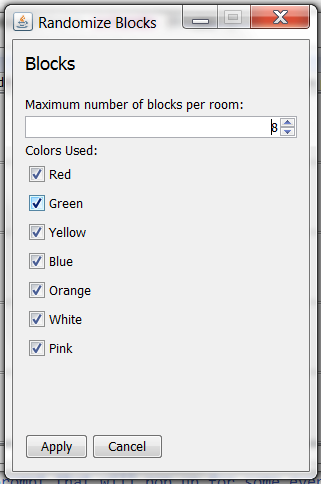
\includegraphics[scale=0.6]{EnvironmentStore/MenuBlocks.png}\\
	Figure 11: The menu appearing when the randomize blocks option is clicked in the menu.
\end{center}
This interface allows the user to specify which block colors they want to be spawned, and also the max. amount of blocks in a room. The interface for random sequence generation is slightly different, and is as follows:
\begin{center}
	\centering
	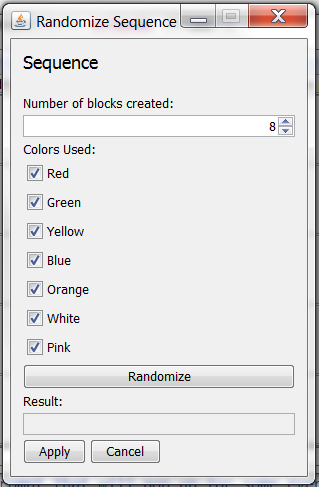
\includegraphics[scale=0.6]{EnvironmentStore/MenuSeq.png}\\
	Figure 12: The menu appearing when the randomize blocks option is clicked in the menu.
\end{center}
The differences between this interface and the previous interface are the Randomize button and Result label, that  create and display resp. the random sequence, and the apply and cancel button which enter the sequence in the map or cancel the creation of the sequence, respectively.


\subsection{Manual editing of Maps}
It is also possible to manually edit a map as it is a plain text XML file.
\begin{enumerate}
\item Copy an existing map file in the $<$SERVER$>/$maps folder to a new file \footnotemark[1].
\item Open the copied map with a text editor. You can then edit the colors in the rooms. Each $<$blocks$>$COL$</$blocks$>$ line inside a $<$zones$>$ of type ROOM adds another block to the room. The currently available colors are BLUE, ORANGE, RED, WHITE, GREEN, YELLOW AND PINK. A room has place for at most 10 blocks.
\item You can change the number of rooms by adding or removing $<$zones$>$ of type ROOM and position the rooms correctly on the map by editing the $<$x$>$ $<$y$>$ $<$width$>$ and $<$height$>$ inside the room's $<$boundingbox$>$. Also you need to add a $<$door$>$ properly positioned on the border of the room.
\item You can edit the goal sequence by adding $<$sequence$>$ items to the map, with colors as mentioned above.
\item You can prevent multiple entities to enter corridor zones by putting true in the item $<$oneBotPerCorridorZone$>$ in the map.
\item You can add entities to the environment by creating more $<$entities$>$ items. Make sure they have a unique $<$name$>$ and that their start position is in a different $<$zone$>$ if you have $<$oneBotPerCorrridorZone$>$ set to true.
\item You can let the server pick a random sequence of a given length by setting the $<$randomSequence$>$ to a positive value. These random blocks are added to the existing sequence items and the random blocks are placed randomly on the map.
\item You can let the server pick random extra blocks to be placed in the rooms on the map by putting a positive number in the $<$randomBlocks$>$ in the map. Note that this addition is on top of all blocks that are already placed in the map; so normally you leave the room zones empty when using this option.
\item You can set per-zone visibility of the zone namelabel in the server map renderer, using a $<$renderOptions$>$ $<$labelVisible$>$ false $</$labelVisible$>$ $</$renderOptions$>$ block to disable visibility.
\item Save the map in the $<$SERVER$>/$maps directory.
\item Edit the map initialization parameter for the server to your new map file. See the section on customizing the server settings. If you now start the server and your new map should be loaded.
\end{enumerate}




\newpage
\section{Scenario Editor}


\subsection{Introduction}
This chapter describes how to make use of the Scenario Editor (Figure \ref{ScenarioEditor}). When you open the editor, you see two main parts:
\begin{enumerate}
\item The Configuration panel, which is used to create, open and save configuration files.
\item The Entity panel, where a list of bots and a list of e-partners are being displayed. Here you can create, modify, rename and delete bots and e-partners.
\end{enumerate}

\begin{figure}[h]
\begin{center}
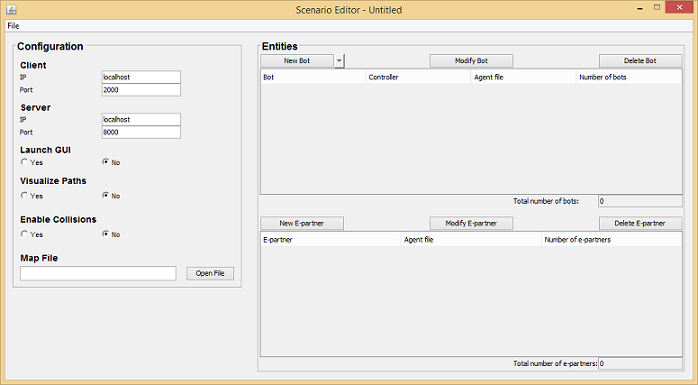
\includegraphics[width=0.9\textwidth]{ScenarioEditor/editor.png}
\caption{Scenario Editor}
\label{ScenarioEditor}
\end{center}
\end{figure}

\subsection{General use}
At the top of the editor you can see a $File$ menu. If you click on that, you get the options to create a new configuration, open an existing configuration, save your configuration, export your configuration and to exit the editor.

On the left side of the editor you can configure a scenario as you like. The Client IP, the Client Port, the Server IP and the Server Port should already contain the default values. You can change them if you need to. You can also indicate whether you want to open a GUI, visualise the paths the bots take or enable collisions. If you have a map file you want to use, you can import it by selecting the $Open$ $file$ button at the right section.

On the right side of the editor you can create, modify, rename and delete bots and e-partners. There also are a list of bots and a list of e-partners that are created, and below each list there is an indication of how many bots or e-partners are created in total.

Linked to the Scenario Editor are the Bot Store and the E-partner Store, which will also be discussed in this document.


\subsection{Configuration Panel}

% wrap figure does not play nice with item lists. But the alternative, having the pic just in the top
% of the page, is taking more space in the end.
\begin{wrapfigure}{r}{0.3\textwidth}
 \begin{center}
	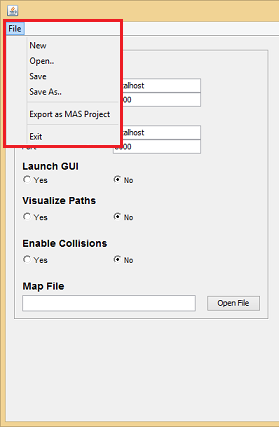
\includegraphics[width=0.3\textwidth]{ScenarioEditor/config.png}
 \end{center}
\caption{Configuration Panel}
\label{fig:ScenarioConfigPanel}
\end{wrapfigure}


A picture of the configuration panel can be found in Figure \ref{fig:ScenarioConfigPanel}. You have the following options:



\begin{itemize}

\item{New configuration file}:
To create a new configuration file, select $File$ $\to$ $New$ in the menu bar. You will now get a new configuration with the default values. Creating a new configuration will reset all previous changes you have made, so make sure you save your current configuration first if you want to keep it.


\item{Open configuration file}:
To open an existing configuration file, select $File$ $\to$ $Open$ in the menu bar. A window will pop up where you can select the folder where the configuration file is saved to. Once you have selected the right folder, select the file and click the $Open$ button.

\item{Save configuration file}:
To save your configuration file, select $File$ $\to$ $Save$ in the menu bar. If your file hasn't been saved before, a window will pop up where you can select the folder you want to save your configuration file to and enter the file name you want to use. Once you have selected the right folder and entered the file name, click the $Save$ button.

\item{Save configuration file as}:
To save your configuration in a new file, select $File$ $\to$ $Save$ $As$ in the menu bar. A window will pop up where you can select the folder you want to save your configuration file to and enter the file name you want to use. Once you have selected the right folder and entered the file name, click the $Save$ button.

\item{Export configuration to mas2g}:
To export your configuration to mas2g, you have to have saved your configuration first. Once you have done that, select $File$ $\to$ $Export$ $as$ $MAS$ $project$ in the menu bar. A window will pop up where you can select the folder you want to export the configuration to and the file name you want to use. Once you have selected the right folder and entered the file name, click the $Export$ $MAS$ $project$ button.

\item{Exit the Scenario Editor}:
If you want to close the Scenario Editor, select $File$ $\to$ $Exit$ in the menu bar. Closing the Scenario Editor will not save any changes you have made, so make sure you save your configuration first if you want to keep it.
\end{itemize}



\subsection{Entity Panel}
The entity panel exists of 2 parts; the top part shows the bot options and the bottom part shows the e-partner options. A picture of the entity panel can be found in Figure \ref{fig:EntityPanel}. You have the following options:


\begin{figure}
\begin{center}
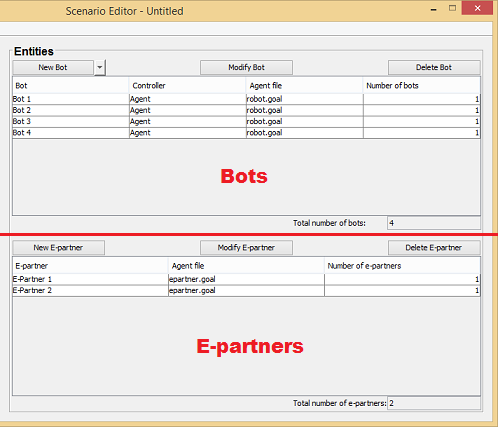
\includegraphics[width=0.6\textwidth]{ScenarioEditor/bot.png}
\end{center}
\caption{Entity Panel}
\label{fig:EntityPanel}
\end{figure}

\begin{itemize}
\item{Create new bot}:
To create a new bot, click the $New$ $Bot$ button. A new bot will appear in the bot list.\\
If you want to create a standard bot (which already has default values), click on the arrow next to the $New$ $Bot$ button. A menu will drop down where you can select one of the standard bots. If you click on one of the standard bots, the bot will appear in the bot list.

\item{Modify bot}:
To modify a bot, select the bot you want to modify in the bot list and click the $Modify$ $Bot$ button. The Bot Store will open in a new window where you can modify the properties of the bot.

\item{Rename bot}:
To rename a bot, you can either use the $Modify$ $Bot$ button to rename in the Bot Store, or you can rename in the Scenario Editor. To rename in the Scenario Editor, select the bot you want to rename in the list with bots. Double click the its name and enter a new name.

\item{Change controller type}:
To change how a bot is controlled, you can either use the $Modify$ $Bot$ button to change it in the Bot Store, or you can change it in the Scenario Editor. To change the controller type in the Scenario Editor, select the bot you want to change and click on its controller type. You should now be able to choose the controller type.

\item{Change the amount of entities of a bot}:
To change how many entities of a type of bot you want, you can either use the $Modify$ $Bot$ button to change it in the Bot Store, or you can change it in the Scenario Editor. To change the entity amount in the Scenario Editor, select the bot that you want to change the amount of. Now double click the amount given, and enter a new number.

\item{Delete bot}:
To delete a bot, select the bot you want to delete in the list with bots and click the $Delete$ $Bot$ button.

\item{Create new e-partner}:
To create a new e-partner, click the $New$ $E$-$partner$ button. A new e-partner will appear in the e-partner list.

\item{Modify e-partner}:
To modify an e-partner, select the e-partner you want to modify in the e-partner list and click the $Modify$ $E$-$partner$ button. The E-partner Store will open in a new window where you can modify the properties of the e-partner.

\item{Rename e-partner}:
To rename an e-partner, you can either use the $Modify$ $E-partner$ button to rename in the E-partner Store, or you can rename in the Scenario Editor. To rename in the Scenario Editor, select the e-partner you want to rename in the list with e-partners. Double click its name and enter a new name.

\item{Change the amount of entities of an e-partner}:
To change how many entities of a type of e-partner you want, you can either use the $Modify$ $E-partner$ button to change it in the E-partner Store, or you can change it in the Scenario Editor. To change the amount in the Scenario Editor, select the e-partner that you want to change the amount of. Now double click the amount given, and enter a new number.

\item{Delete e-partner}:
To delete an e-partner, select the e-partner you want to delete in the e-partner list and click the $Delete$ $E$-$partner$ button.

\end{itemize}


\subsection{Bot Store}
Figure \ref{fig:BotStore} shows a picture of the Bot Store. You have the following options:

\begin{figure}
\begin{center}
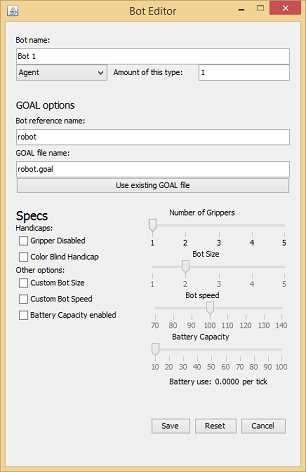
\includegraphics[width=0.4\textwidth]{ScenarioEditor/bs.png}
\end{center}
\caption{Bot Store}
\label{fig:BotStore}
\end{figure}

\begin{itemize}
\item{Rename bot}:
To rename a bot, click on the field that contains its current name. Now you are able to edit the current name or you can enter a new name.

\item{Change controller type}:
To change how a bot is controller, you can click on its current controller type. Now you are able to choose the controller type.

\item{Change the amount of entities}:
To change how many entities of the bot you want, you can click on the field that contains the current number of entities. Now you are able to edit the amount.

\item{GOAL options}:
You can enter the GOAL options for your bot under the $GOAL$ $options$ section. Here you can indicate what its reference name in GOAL should be, and you can select a GOAL agent file which will control the bot. To select the GOAL agent file, you can click on the $Use$ $existing$ $GOAL$ $file$ button. A window will pop up where you can select the folder where the GOAL file is saved to. Once you have selected the right folder, select the file and click the $Open$ button.

\item{Bot properties}:
You can find the available bot properties under the $Properties$ section. To change what properties you want the e-partner to have, you can select or deselect the checkbox next to the property description. Once you have enabled a property, you can use the sliders to change the value of that property.

\item{Save modifications}:
If you want to save the changes you have made to the bot, you can click on the $Save$ button. The Bot Store window will close, and your changes will have been saved.

\item{Reset modifications}:
If you want to reset the changes you have made to the bot, you can click on the $Reset$ button. Your changes will have been reverted to the last saved configuration.

\item{Cancel modifications}:
If you want to cancel modifying the bot without saving any changes, you can click on the $Cancel$ button. The Bot Store window will close.
\end{itemize}


\subsection{E-partner Store}
WARNING: The e-partner component of BW4T is not yet completely ready for use.

A picture of the E-partner Store is shown in Figure \ref{fig:epartnerstore}. You have the following options:

\begin{figure}[h]
\begin{center}
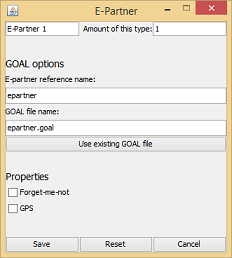
\includegraphics[width=0.4\textwidth]{ScenarioEditor/es.png}
\end{center}
\caption{E-partner Store}
\label{fig:epartnerstore}
\end{figure}

\begin{itemize}
\item{Rename e-partner}:
To rename an e-partner, click on the field that contains its current name. Now you are able to edit the current name or you can enter a new name.

\item{Change the amount of entities}:
To change how many entities of the e-partner you want, you can click on the field that contains the current number of entities. Now you are able to edit the amount.

\item{GOAL options}:
You can enter the GOAL options for your e-partner under the $GOAL$ $options$ section. Here you can indicate what its reference name in GOAL should be, and you can select a GOAL agent file which will control the e-partner. To select the GOAL agent file, you can click on the $Use$ $existing$ $GOAL$ $file$ button. A window will pop up where you can select the folder where the GOAL file is saved to. Once you have selected the right folder, select the file and click the $Open$ button.

\item{E-partner properties}:
You can find the available e-partner properties under the $Properties$ section. To change what properties you want the e-partner to have, you can select or deselect the checkbox next to the property description.

\item{Save modifications}:
If you want to save the changes you have made to the e-partner, you can click on the $Save$ button. The E-partner Store window will close, and your changes will have been saved.

\item{Reset modifications}:
If you want to reset the changes you have made to the e-partner, you can click on the $Reset$ button. Your changes will have been reverted to the last saved configuration.

\item{Cancel modifications}:
If you want to cancel modifying the e-partner without saving any changes, you can click on the $Cancel$ button. The E-partner Store window will close.

\end{itemize}

\end{document}
